\documentclass[11pt]{article}
\usepackage[margin=0.87in]{geometry}
\usepackage[T1]{fontenc}
\usepackage{lmodern}
\usepackage{microtype}
\usepackage{amsmath,amssymb}
\usepackage{booktabs}
\usepackage{graphicx}
\usepackage{xcolor}
\usepackage{hyperref}
\usepackage{tikz}
\usetikzlibrary{arrows.meta,positioning}
\usepackage{pgfplots}
\pgfplotsset{compat=1.18}
\hypersetup{colorlinks=true,linkcolor=blue!50!black,urlcolor=blue!50!black}
\definecolor{sourceblue}{HTML}{087E9B}
\definecolor{graphpurple}{HTML}{6155A4}
\definecolor{siteamber}{HTML}{B47012}

\title{SemDAG: A Controlled Evaluation of Lexical and Graph Retrieval for Code Agents\\[0.45em]
\large\normalfont Auditing a graph-first localizer and measuring BM25-seeded typed walks on 129 public edit-site tasks}
\author{Stewart Barteau\\Independent Researcher}
\date{November 2026}

\begin{document}
\maketitle

\begin{abstract}
We evaluate whether repository structure helps a small code agent locate edit sites after the issue has been matched against live function source. SemDAG builds a typed graph of files, classes, functions, calls, and imports, then uses BM25 function scores as the restart distribution of a short graph walk. We evaluate the production retriever on 129 public competition tasks, of which 116 admit a function-level gold site and 128 admit a file-level gold site. At function Hit@5, BM25 reaches 58/116 and the selected SemDAG walk reaches 56/116 (paired difference $-1.7$ percentage points; 95\% bootstrap interval $[-7.8,4.3]$). At function Hit@10, the counts are 68 and 69; at file Hit@10, they are 108/128 and 111/128. A disjoint 42-task pool ties at function Hit@5 (20 each). Greater walk damping reduces overall Hit@5. The graph therefore supplies limited file-level context under this protocol, while the measured function-level difference remains unresolved. Integrity checks pass on all 129 full task snapshots. These are retrieval results; the current SemDAG agent has not yet had a paired end-to-end evaluation.
\end{abstract}

\section{Introduction}
Finding a likely edit site is a distinct problem from producing a correct patch. A code agent must use a short issue statement to prioritize a small portion of a much larger codebase. Lexical source search directly measures vocabulary overlap, while a call and containment graph can connect nearby code with different wording. The question is whether that structural step improves localization when the query already reads source text.

SemDAG combines the two signals in a fixed order: query live function source, use the resulting BM25 scores as a probability distribution, then walk a typed structural graph lightly. This paper evaluates that production algorithm against its zero-walk lexical baseline. All reported retrieval arms use the same candidate admission rule, and the measurement imports the retriever that ships with the agent. We examine function and file coverage separately, including a held-out task pool and a paired uncertainty estimate.

\begin{figure}[t]
\centering
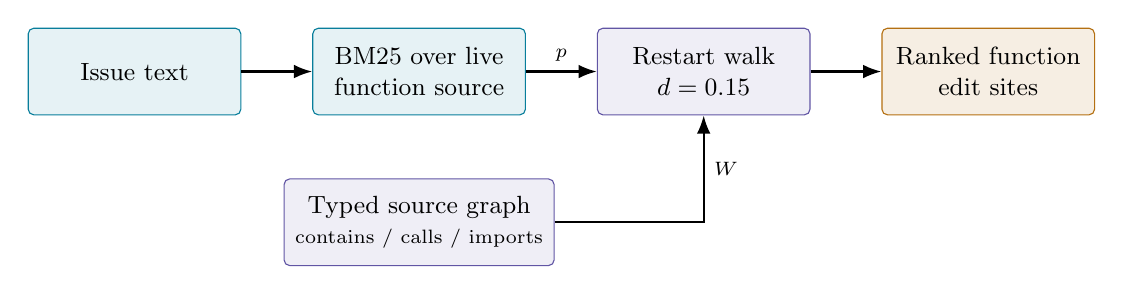
\begin{tikzpicture}[>=Latex, node distance=8mm and 9mm, every node/.style={font=\small}]
\tikzstyle{box}=[draw,rounded corners=2pt,align=center,minimum height=11mm,minimum width=27mm,inner sep=4pt]
\node[box,fill=sourceblue!10,draw=sourceblue] (issue) {Issue text};
\node[box,fill=sourceblue!10,draw=sourceblue,right=of issue] (bm) {BM25 over live\\function source};
\node[box,fill=graphpurple!10,draw=graphpurple,below=of bm] (ir) {Typed source graph\\\scriptsize contains / calls / imports};
\node[box,fill=graphpurple!10,draw=graphpurple,right=of bm] (walk) {Restart walk\\$d=0.15$};
\node[box,fill=siteamber!12,draw=siteamber,right=of walk] (rank) {Ranked function\\edit sites};
\draw[->,thick] (issue) -- (bm);
\draw[->,thick] (bm) -- node[above,font=\scriptsize] {$p$} (walk);
\draw[->,thick] (ir.east) -| node[pos=.75,right,font=\scriptsize] {$W$} (walk.south);
\draw[->,thick] (walk) -- (rank);
\end{tikzpicture}
\caption{Production SemDAG. The same snapshot supplies function source and the typed graph. Only functions with positive lexical scores are eligible for the returned ranking; the walk reorders them using structural context.}
\label{fig:pipeline}
\end{figure}

\section{Method}
\subsection{Snapshot and typed graph}
A deterministic snapshot records Python files and verifies a tree hash computed in globally sorted path order. The AST front end records file, class, function, and method nodes, including asynchronous functions and exact source spans. Lexical nesting produces \texttt{contains} edges. Statically justified call targets produce \texttt{calls} edges; same-module definitions, \texttt{self}/\texttt{cls}, class-qualified names, and imported symbols are handled conservatively. Imports resolved to files in the snapshot produce \texttt{imports} edges. Ambiguous names and dynamic dispatch are left unresolved rather than connected to an arbitrary same-named function.

Test files, generated harness wrappers, and the bundled localization implementation are excluded from both candidate ranking and graph traversal. This admission rule is shared by every primary comparison arm. The integrity check returns no ranking if the snapshot hash fails.

\subsection{Lexical restart and structural walk}
The issue is tokenized into identifiers and their snake-case and camel-case parts. Function source supplies BM25 terms; path and qualified-name terms receive a fixed threefold repetition. We use $k_1=1.2$ and $b=0.75$. Let $s_i$ be the BM25 score of eligible function $i$. Positive scores define the restart distribution
\begin{equation}
 p_i = \frac{s_i\,\mathbf{1}[s_i>0]}{\sum_j s_j\,\mathbf{1}[s_j>0]}.
\end{equation}
The walk uses undirected versions of resolved \texttt{contains}, \texttt{calls}, and \texttt{imports} edges with unit relation weight. Let $W$ be the row-normalized adjacency; dangling mass returns to $p$. Starting from $r^{(0)}=p$, SemDAG applies 30 iterations of
\begin{equation}
 r^{(t+1)}=(1-d)p+dW^\top r^{(t)},
 \label{eq:walk}
\end{equation}
with the dangling-mass correction included in the restart term. The selected production setting is $d=0.15$. At $d=0$, the ranking is exactly BM25; the measurement asserts this task by task. Final sorting uses full-precision scores and a deterministic file-and-line tie-break. Only positive-BM25 functions are returned, so graph diffusion changes their order rather than adding unmatched functions.

\section{Evaluation protocol}
The dataset contains 129 public competition tasks spanning four codebases. Issue text is the query. Hints and test patches are not read; reference patches are used only to construct gold sites and score rankings. A gold function is the innermost pre-patch function covering a deleted line, or, for a pure insertion, covering both old-side neighbors. This yields 438 gold functions over 116 evaluable tasks. File-level gold sites exist for 128 tasks. No function gold site lies in an excluded test file.

Hit@$k$ counts tasks with any gold function or file among the first $k$ returned candidates. The reported setting was chosen on a 74-task selection pool; a disjoint 42-task function-level pool is reported separately and was not used to choose it. Paired task-level bootstrap intervals use 4{,}000 resamples, seed 0. The primary control is the same BM25 document construction and candidate set at $d=0$. Additional damping values isolate the effect of graph diffusion.

\section{Results}
\subsection{Localization and damping}
\begin{table}[t]
\centering
\caption{All-task localization. Function columns use 116 tasks; file Hit@10 uses 128. Counts are tasks with at least one gold site in the top $k$.}
\label{tab:main}
\begin{tabular}{lrrrr}
\toprule
Method & Function @1 & Function @5 & Function @10 & File @10 \\
\midrule
BM25 ($d=0$) & 21 & 58 & 68 & 108 \\
SemDAG ($d=0.15$) & 19 & 56 & 69 & \textbf{111} \\
SemDAG ($d=0.30$) & 14 & 52 & \textbf{72} & 109 \\
SemDAG ($d=0.50$) & 16 & 45 & 68 & 110 \\
SemDAG ($d=0.85$) & 11 & 33 & 53 & 109 \\
\bottomrule
\end{tabular}
\end{table}

\begin{figure}[t]
\centering
\begin{minipage}{0.50\linewidth}
\centering
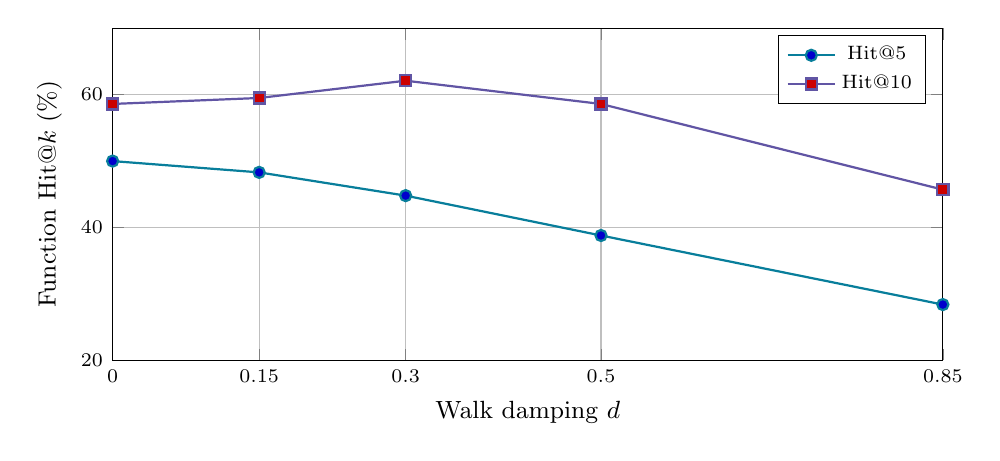
\begin{tikzpicture}
\begin{axis}[width=\linewidth,height=5.8cm,xlabel={Walk damping $d$},ylabel={Function Hit@$k$ (\%)},xmin=0,xmax=.85,ymin=20,ymax=70,xtick={0,.15,.30,.50,.85},grid=major,legend style={font=\scriptsize,at={(0.98,0.98)},anchor=north east},tick label style={font=\scriptsize},label style={font=\small}]
\addplot+[thick,mark=*,color=sourceblue] coordinates {(0,50.0)(.15,48.3)(.30,44.8)(.50,38.8)(.85,28.4)};
\addlegendentry{Hit@5}
\addplot+[thick,mark=square*,color=graphpurple] coordinates {(0,58.6)(.15,59.5)(.30,62.1)(.50,58.6)(.85,45.7)};
\addlegendentry{Hit@10}
\end{axis}
\end{tikzpicture}
\end{minipage}\hfill
\begin{minipage}{0.47\linewidth}
\centering
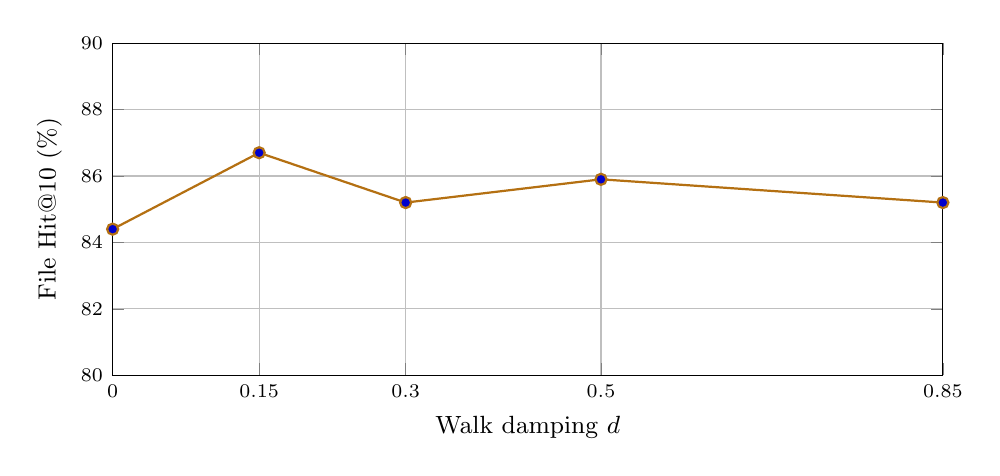
\begin{tikzpicture}
\begin{axis}[width=\linewidth,height=5.8cm,xlabel={Walk damping $d$},ylabel={File Hit@10 (\%)},xmin=0,xmax=.85,ymin=80,ymax=90,xtick={0,.15,.30,.50,.85},ytick={80,82,84,86,88,90},grid=major,tick label style={font=\scriptsize},label style={font=\small}]
\addplot+[thick,mark=*,color=siteamber] coordinates {(0,84.4)(.15,86.7)(.30,85.2)(.50,85.9)(.85,85.2)};
\end{axis}
\end{tikzpicture}
\end{minipage}
\caption{Measured damping sweep using the production retriever. The left denominator is 116 tasks and the right denominator is 128. The right panel uses a narrower, explicitly labeled vertical scale to show the small file-level differences. Percentages are plotted from the integer counts in Table~\ref{tab:main}.}
\label{fig:damping}
\end{figure}

At function Hit@5 the selected walk trails BM25 by two tasks: a paired difference of $-0.0172$ with 95\% interval $[-0.0776,0.0431]$. At function Hit@10 it leads by one task, and at file Hit@10 by three. These observations do not establish a function-level advantage. Larger damping raises function Hit@10 at $d=0.30$ but lowers Hit@5, so a single recall number obscures the ranking tradeoff.

\subsection{Held-out tasks and paired uncertainty}
On the 42-task held-out function-level pool, BM25 and $d=0.15$ both reach 20 at Hit@5; at Hit@10 the counts are 24 and 26. The paired Hit@5 difference is 0 with 95\% interval $[-0.0714,0.0714]$. A larger $d=0.50$ reaches 23 at Hit@5 and 28 at Hit@10 in this pool, but this value was not selected on it. The contrast shows that the useful damping may vary with the task distribution.

\begin{figure}[t]
\centering
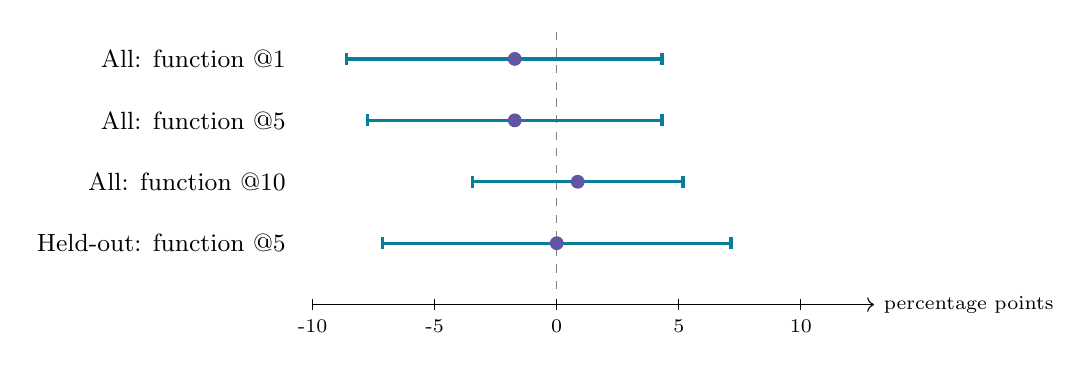
\begin{tikzpicture}[x=0.31cm,y=0.78cm,font=\small]
\draw[->] (-10,0) -- (13,0) node[right,font=\scriptsize] {percentage points};
\foreach \x in {-10,-5,0,5,10} {\draw (\x,0.09)--(\x,-0.09) node[below,font=\scriptsize] {\x};}
\draw[dashed,gray] (0,0.25)--(0,4.5);
\node[anchor=east] at (-10.7,4) {All: function @1};
\node[anchor=east] at (-10.7,3) {All: function @5};
\node[anchor=east] at (-10.7,2) {All: function @10};
\node[anchor=east] at (-10.7,1) {Held-out: function @5};
\foreach \lo/\mid/\hi/\y in {-8.62/-1.72/4.31/4,-7.76/-1.72/4.31/3,-3.45/0.86/5.17/2,-7.14/0/7.14/1} {
  \draw[very thick,sourceblue] (\lo,\y)--(\hi,\y);
  \draw[very thick,sourceblue] (\lo,\y-.10)--(\lo,\y+.10);
  \draw[very thick,sourceblue] (\hi,\y-.10)--(\hi,\y+.10);
  \fill[graphpurple] (\mid,\y) circle[radius=2.5pt];
}
\end{tikzpicture}
\caption{Paired SemDAG-minus-BM25 differences with 95\% task-bootstrap intervals. All four intervals include zero; the plot reports uncertainty rather than a superiority claim.}
\label{fig:ci}
\end{figure}

\subsection{Integrity and implementation checks}
The repaired snapshot and parity check agree on all 129 full task snapshots, and the integrated localizer returns candidates on all 129. A separate adversarial fixture checks import and call resolution, duplicate names, test and tool-path exclusion, determinism, and use of all three edge relations. The measurement imports the same production \texttt{retriever.py} as the agent package; its zero-damping assertion protects the BM25 comparison from an implementation mismatch.

\section{Discussion and limitations}
The source query supplies the main ranking signal. A light graph walk preserves near-parity at function level and moves three additional gold files into the top ten on this public set. The file-level count is small, and no paired confidence interval for that particular contrast is claimed here. More aggressive diffusion is not uniformly useful. Because only functions with positive BM25 scores can be returned, the present design cannot rescue an edit site whose source and metadata share no query terms.

The AST graph is deliberately incomplete: dynamic dispatch and runtime imports are unresolved. Function-level scoring excludes module-level and newly added code; 13 of 129 tasks have no function-level gold site. These public tasks span four codebases, so the result need not generalize to unseen distributions. The current SemDAG package has passed directory validation and localization checks, but no paired agent-resolution experiment has been run for this exact production retriever. We therefore make no claim that the walk improves patch correctness or resolved-task rate.

\section{Reproducibility}
The production package is at \path{AgenticSubmission/v4_semdag/skills/semdag/}. The evaluation script \path{PaperTrack/phase4_semdag/measure_v2.py} writes the task-level results and summary to \path{PaperTrack/phase4_semdag/out/}; the reported counts and intervals come from \path{v2_summary.json}. The integrity run is \path{verify_gate.py}, and the structural contract fixture is \path{adversarial_check.py}. No hidden hints or test patches are used to rank candidates. The graphs in this paper encode the integer counts and paired intervals from those on-disk receipts.

\begin{thebibliography}{9}
\bibitem{robertson2009} S. Robertson and H. Zaragoza. The Probabilistic Relevance Framework: BM25 and Beyond. \emph{Foundations and Trends in Information Retrieval}, 2009. DOI: 10.1561/1500000019.
\bibitem{haveliwala2002} T. Haveliwala. Topic-Sensitive PageRank. \emph{Proceedings of the 11th International World Wide Web Conference}, 2002. DOI: 10.1145/511446.511513.
\end{thebibliography}

\end{document}
